
%(BEGIN_QUESTION)
% Copyright 2007, Tony R. Kuphaldt, released under the Creative Commons Attribution License (v 1.0)
% This means you may do almost anything with this work of mine, so long as you give me proper credit

In measurement and control systems, there is often a need to modify or select instrumentation signals.  Devices designed to perform calculations on instrument signals are called {\it computing relays}, and digital algorithms inside control computers designed with the same tasks in mind are called {\it function blocks}.

Identify the functions of each relay (or function block) shown here:

$$\includegraphics[width=15.5cm]{i01781x01.eps}$$

\underbar{file i01781}
%(END_QUESTION)





%(BEGIN_ANSWER)

$$\includegraphics[width=15.5cm]{i01781x02.eps}$$

%(END_ANSWER)





%(BEGIN_NOTES)


%INDEX% Relay, computational: symbol identification

%(END_NOTES)


